\documentclass[conference]{IEEEtran}
\IEEEoverridecommandlockouts
\usepackage{cite}
\usepackage{amsmath,amssymb,amsfonts}
\usepackage{algorithmic}
\usepackage{graphicx}
\usepackage{textcomp}
\usepackage{xcolor}
\usepackage{url}

\def\BibTeX{{\rm B\kern-.05em{\sc i\kern-.025em b}\kern-.08em
    T\kern-.1667em\lower.7ex\hbox{E}\kern-.125emX}}

\begin{document}

\title{Adaptive Explanation Obfuscation via Reinforcement Learning}

\author{\IEEEauthorblockN{1\textsuperscript{st} Gamze Erdo\u{g}an}
\IEEEauthorblockA{\textit{Istanbul Technical University}\\
Istanbul, T\"urkiye \\
gamze.erdogan@itu.edu.tr}
\and
\IEEEauthorblockN{2\textsuperscript{nd} Prof. Enver \"Ozdemir}
\IEEEauthorblockA{\textit{Istanbul Technical University}\\
Istanbul, T\"urkiye \\
ozdemiren@itu.edu.tr}
\and
\IEEEauthorblockN{3\textsuperscript{rd} Bet\"ul G\"uven\c{c} Paltun}
\IEEEauthorblockA{\textit{Ericsson}\\
Istanbul, T\"urkiye \\
betul.guvenc.paltun@ericsson.com}
\and
\IEEEauthorblockN{4\textsuperscript{th} Leyli Kara\c{c}ay}
\IEEEauthorblockA{\textit{Ericsson}\\
Istanbul, T\"urkiye \\
leyli.karacay@ericsson.com}
}

\maketitle

\begin{abstract}
The solution introduces a reinforcement learning (RL) agent that functions as a protective layer around an Explainable Artificial Intelligence (XAI) model, dynamically adjusting the level of explanation provided based on ongoing interactions. The problem is structured as a continuous adversarial min-max game: an adversary attempts to reconstruct a surrogate model using the explanations given, while the RL agent actively obfuscates the explanations to prevent successful extraction. The system aims to satisfy legitimate user needs while penalizing the agent if the adversary successfully predicts or reconstructs the model. Over time, the agent learns to adapt its strategy, minimizing risks while maintaining the usefulness of explanations for authorized users.
\end{abstract}

\begin{IEEEkeywords}
Explainable AI (XAI), Reinforcement Learning (RL), Model Extraction Attacks, Privacy, Obfuscation.
\end{IEEEkeywords}

\section{Introduction}
Explainable Artificial Intelligence (XAI) focuses on making complex models and their predictions interpretable, providing insights into the reasoning processes behind machine learning outputs. However, while offering explanations assists legitimate users in comprehending model behavior, it simultaneously creates potential vulnerabilities that adversaries may leverage to replicate models. 

A model extraction attack occurs when an adversary attempts to replicate a black box model. If an attack utilizes explanations, it is called an explanation-aware model extraction attack (XaMEA). In such attacks, the adversary sends a massive volume of crafted queries to reveal information about the target model's behavior. The explanations consist of additional information such as feature importance or confidence scores, which the attacker uses to match both the outputs and explanations of a surrogate model to those of the target model. If explainability is provided, even highly complex models are vulnerable to these extraction attacks.

To address these challenges, we introduce an approach that integrates a reinforcement learning (RL) agent with XAI to dynamically enhance privacy and security without strictly compromising the explanation quality for benign users.

\section{Related Work}
Security and privacy concerns in AI, particularly regarding model extraction attacks, have prompted the development of explainability methods that aim to balance transparency and protection against adversarial threats. Current static methods to protect models from vulnerabilities involve various trade-offs:

\begin{itemize}
    \item \textbf{Top-$k$ Truncation:} This method limits information leakage by sharing only the most significant outputs, such as the top $k$ features \cite{b2}. While it increases the difficulty for adversaries, it mainly forces them to send a greater number of queries to obtain sufficient data for proper training, rather than fully preventing extraction.
    \item \textbf{Generalization:} Another approach is categorizing values into brackets or rounding decimals to provide fewer specific answers \cite{b3}. However, adversaries can still replicate the surrogate model to mimic these generalized outputs, and the lack of precision compromises the usefulness of the explanations for legitimate users.
    \item \textbf{API Limiting:} Restricting how many queries users can access acts as a safeguard. However, this limitation hinders legitimate users who require detailed queries to fully understand or audit the model's decisions, reducing transparency.
    \item \textbf{Adding Noise:} Intentionally distorting outputs makes it harder to reverse engineer the model, but it compromises the fidelity of the explanation \cite{b4}. This results in a potential loss of interpretability and reliability for legitimate users.
\end{itemize}

Unlike these static methods, our proposed solution utilizes dynamic obfuscation via an RL agent, adapting to user behavior to maintain explainability without compromising privacy.

\section{Proposed System Architecture}
The system consists of an inference provider who manages the ML model along with its associated explainability module. The RL agent acts as a protective mechanism that decides how much information to conceal or modify in an explanation.

\begin{figure}[htbp]
\centerline{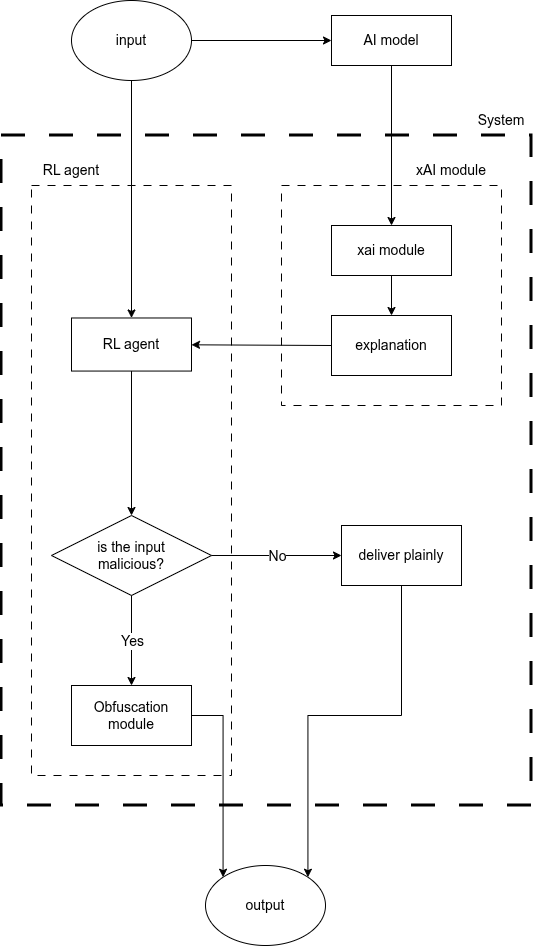
\includegraphics[width=\columnwidth]{fig1_overview.png}}
\caption{High-level overview of the system architecture.}
\label{fig1}
\end{figure}

As illustrated in Fig.~\ref{fig1}, the high-level components of the system are:
\begin{itemize}
    \item \textbf{AI Model:} A model hosted and served by the inference provider.
    \item \textbf{Input:} The query submitted for processing.
    \item \textbf{RL agent:} Determines how much information to conceal in an explanation to limit model extraction while preserving utility.
    \item \textbf{Obfuscation module:} Intentionally obfuscates explanations to prevent attackers from learning too much about the model.
    \item \textbf{XAI module:} Generates explanations for the outputs of the model.
\end{itemize}

\begin{figure}[htbp]
\centerline{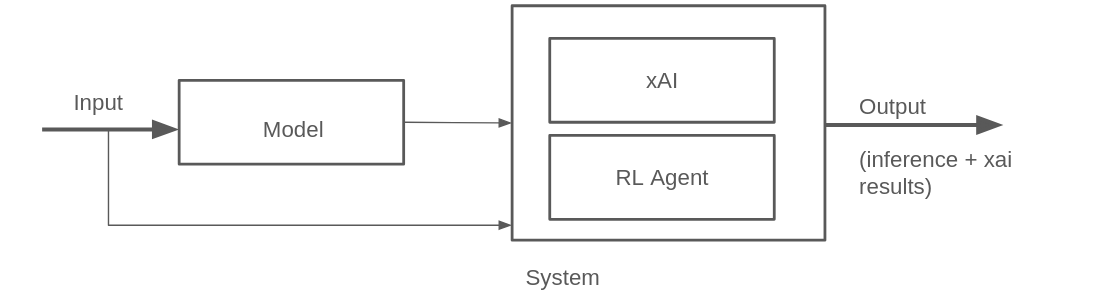
\includegraphics[width=\columnwidth]{fig2_workflow.png}}
\caption{System workflow: inference model output is explained by the XAI module and selectively obfuscated by the RL agent before returning results.}
\label{fig2}
\end{figure}

The workflow operates as follows (see Fig.~\ref{fig2}):
\begin{enumerate}
    \item An input query is submitted to the system.
    \item The input is processed on the model, generating an output.
    \item The input is simultaneously sent to the RL agent for analysis.
    \item The RL agent examines the input's relation to historical queries and determines the degree of obfuscation required.
    \item The XAI module receives the output and generates a baseline explanation, which is sent to the RL agent.
    \item The RL agent decides whether to apply obfuscation to the explanation via the obfuscation module.
    \item The processed output and the (potentially obfuscated) explanation are returned to the user.
\end{enumerate}

\section{Game Design for the RL Agent}
The RL agent is trained using a game-based framework designed to enhance model security while maintaining explanation utility. The setup simulates a continuous adversarial scenario, as depicted in Fig.~\ref{fig3}.

\begin{figure}[htbp]
\centerline{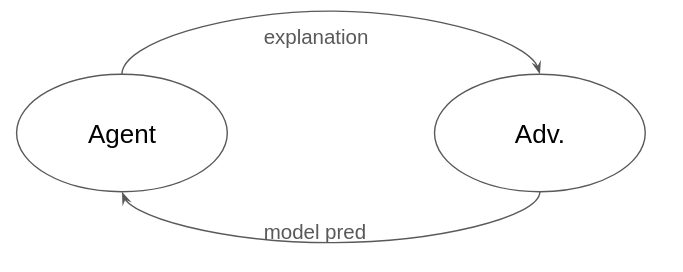
\includegraphics[width=\columnwidth]{fig3_training_loop.png}}
\caption{Game-based training loop: the RL agent obfuscates explanations; the adversary trains a surrogate model, and rewards/penalties are assigned based on security and explanation utility.}
\label{fig3}
\end{figure}

\subsection{Min-Max Game Formulation}
\textbf{Step 1: State at time $t$}\\
The state $s_{i}$ at time $t$ is the history of queries received from a specific user, where $x_{i}$ is the query and $y_{i}$ is the output.
\begin{equation}
s_i = \{(x_1, y_1), (x_2, y_2), \dots, (x_i, y_i)\}
\end{equation}

\textbf{Step 2: RL Agent Action}\\
The RL agent determines an obfuscation function $f_{obfus}$ to apply to the true explanation $E_{true}$. The action $a_t$ is a continuous variable representing the intensity of abstraction:
\begin{equation}
E_{output} = a_t(E_{true})
\end{equation}
If $a_t = 0$, $E_{output} = E_{true}$ (full explanation). If $a_t = 1$, $E_{output}$ is random noise or no explanation (full obfuscation).

\textbf{Step 3: Adversary Action}\\
The adversary leverages $E_{output}$ to construct a surrogate model $S$ targeting the original model $M$. The adversary minimizes the extraction loss $L_{extract}$:
\begin{equation}
\min L_{extract}(S(x), M(x) | E_{output})
\end{equation}

\textbf{Step 4: Reward Function}\\
The reward function $R_t$ balances security (maximizing adversary loss) and utility (minimizing explanation deviation). 
\begin{equation}
R_t = \lambda \cdot L_{extract}(S, M) - \mu \cdot ||E_{true} - E_{output}||
\end{equation}
Where $\lambda$ and $\mu$ are non-negative scalar hyperparameters weighing the importance of model security and explanation fidelity, respectively.

\subsection{Security-Utility Tradeoff}
By adjusting $\lambda$ and $\mu$, the system designer controls the emphasis on security versus utility. High $\lambda$ prioritizes preventing model extraction, forcing the agent to obscure data even if explanation quality drops. High $\mu$ penalizes obfuscation, yielding clear explanations but higher extraction risks. A balanced approach applies obfuscation only as needed to mitigate risk.

\section{Advantages of the Proposed Solution}
The dynamic integration of the RL agent provides several technical benefits:
\begin{itemize}
    \item \textbf{Enhanced Security:} Mitigates model extraction attacks by limiting explanation detail during suspicious activity.
    \item \textbf{Adaptive Explanations:} Continuously monitors query patterns and adapts the detail level based on historical interactions.
    \item \textbf{Balanced Utility:} Unlike static methods, authorized users receive high-quality insights while adversaries are stifled.
    \item \textbf{Robustness:} The RL agent adapts over time, effectively countering evolving attack strategies across varied XAI methods.
\end{itemize}

\begin{thebibliography}{00}
\bibitem{b1} A. Yan, T. Huang, L. Ke, X. Liu, Q. Chen, and C. Dong, ``Explanation leaks: Explanation-guided model extraction attacks,'' \textit{Information Sciences}, vol. 632, pp. 269-284, 2023.
\bibitem{b2} Z. Yue, Z. He, H. Zeng, and J. McAuley, ``Black-box attacks on sequential recommenders via data-free model extraction,'' in \textit{Proc. 15th ACM Conf. Recommender Syst. (RecSys '21)}, New York, NY, USA, 2021, pp. 44-54.
\bibitem{b3} F. Tram\`er, F. Zhang, A. Juels, M. K. Reiter, and T. Ristenpart, ``Stealing machine learning models via prediction APIs,'' in \textit{Proc. 25th USENIX Security Symp. (USENIX Security 16)}, Austin, TX, USA, 2016, pp. 601-618.
\bibitem{b4} S. Saifullah, D. Mercier, A. Lucieri, A. Dengel, and S. Ahmed, ``The privacy-explainability trade-off: unraveling the impacts of differential privacy and federated learning on attribution methods,'' \textit{Front. Artif. Intell.}, vol. 7, art. no. 1236947, Jul. 2024.
\end{thebibliography}

\end{document}
